\FloatBarrier
\chapter{Solution Design}
\label{sec:solution}
\section{Requirements}
\label{sec:solution:req}
\subsection{Context and Goal}
First, the context and objectives of the solution design are defined. The system is provided as a web-based application, as illustrated in Figure~\ref{fig:sol_context}. The target users include both process modeling experts and domain experts who need to create process models from textual documents. To improve modeling efficiency and support non-expert users, the system leverages the LLM service of AutoBPMN.AI for automated model generation. The overall objective is to provide an integrated platform in which users can complete the entire modeling workflow—from document upload to model creation, modification, and subsequent management—in a seamless and user-friendly manner, thereby addressing RQ2.
\begin{figure}[htb!]
  \centering
  \caption{System context} 
  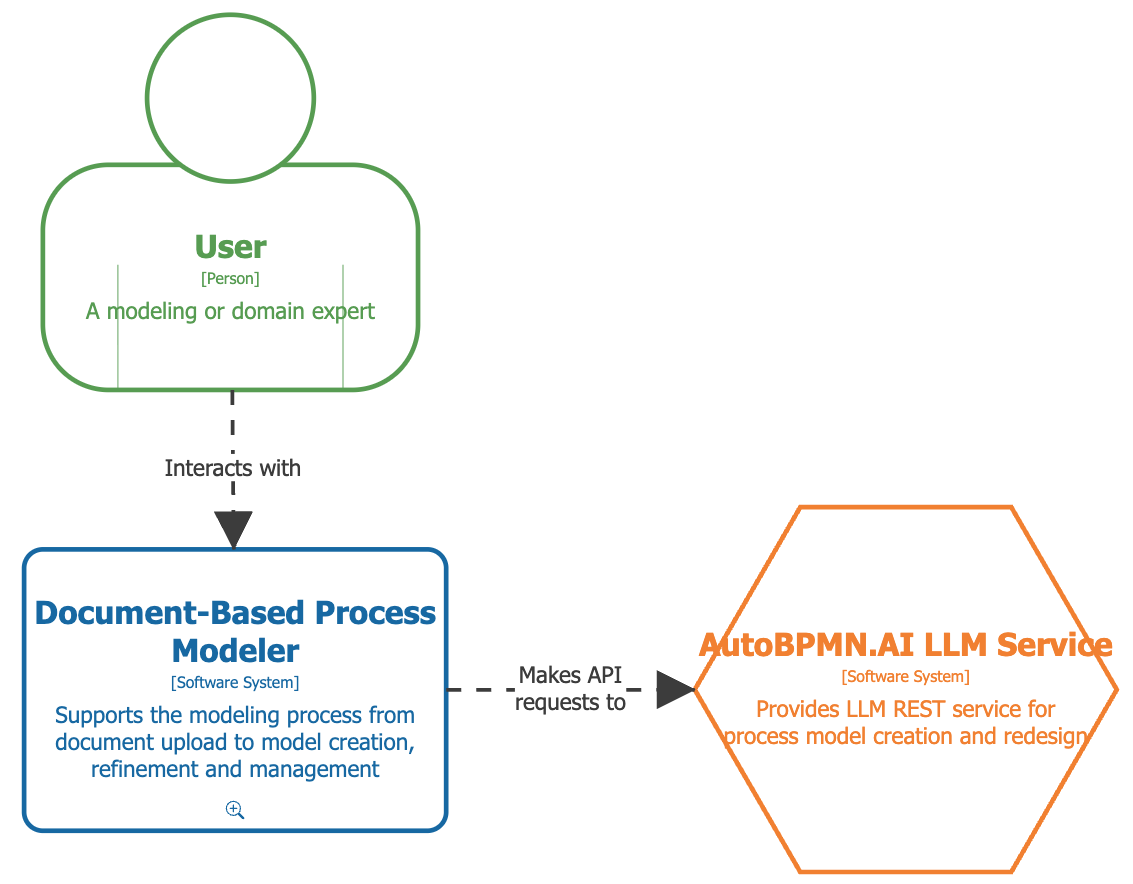
\includegraphics[width=0.8\textwidth]{images/sol_context.png}
  \label{fig:sol_context}
\end{figure}

\subsection{Requirements Elicitation}
Functional requirements define the system’s expected behavior by describing the functions, inputs, outputs, and interactions that enable the system to fulfill its intended objectives \cite{functional_requirement_wiki}. In this work, we adopt the classification proposed by \cite{randall1988service}, further diving the functional requirements into minimal requirements, which represent the indispensable core functionalities required for the system to operate, and enhancing requirements, which include additional features that improve usability and overall performance but are not strictly necessary for basic operation.

When starting the work, the following minimal requirements for the system have been elicitated by my supervisor. Firstly, the system should allow users to upload multiple documents. The basic process modelling is defined as follows: first, the user should be able to select multiple passages from a single document; then, by clicking a Generate button, the system will send the selected text to the LLM service. The system should then display the generated model side-by-side with the document to facilitate verification. Besides, the system should always provide a clear visual link between the text and the generated model. Then a user should be able to select other passages to create more models. Another important requirement is that the system should allow users to establish process-subprocess relationships between models. This flow should be designed on a single web page to avoid users having to switch between tools. The activities described are depicted in the Figure~\ref{fig:workspace_usage_model}. Here, we use the concept of workspace for this dedicated interface, a term commonly used across many software tools, where the modeling flow is performed. 
\begin{figure}[htb!]
  \centering
  \caption{Usage model} 
  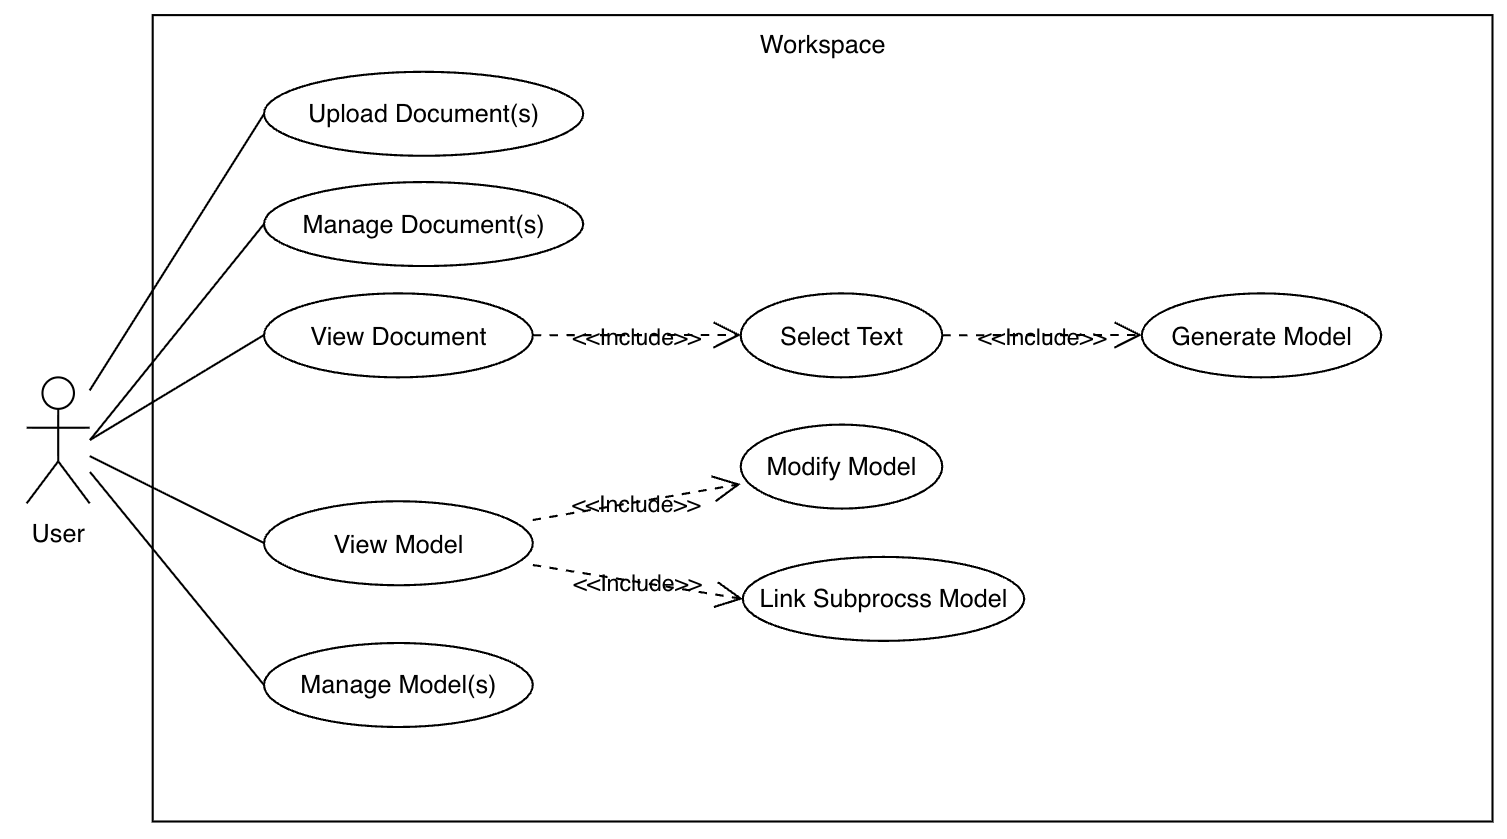
\includegraphics[width=1\textwidth]{images/sol_workspace_interaction_usage_model.png}
  \label{fig:workspace_usage_model}
\end{figure}

Regarding non-functional requirements, only usability, as a very general goal, is defined at this stage. Besides this, a series of technical design constraints are specified. In addition to the two constraints already introduced in the system context, i.e. the system should be implemented as a web-based application and should leverage AutoBPMN.AI’s LLM service\footnote{\url{https://autobpmn.ai/}, accessed 2026-04-15}, two more constraints are explicitly defined. First, the frontend should be developed using native web technologies (JavaScript, HTML, and CSS). Second, the visualization of the process model should be implemented using the CPEE Layout\footnote{\url{https://github.com/etm/cpee-layout}, accessed 2026-04-15} library, following the same layout as used in AutoBPMN.AI, which makes the models easy to export and import, and also provides the potential for them to be uploaded to the CPEE environment without additional manual effort, where they can be directly further manipulated and executed.

With the development of the system, several enhancing requirements were identified. One key aspect is model modification, since generated models are not final and need to be refined. The system therefore supports several ways to modify models. Users can edit the model manually, provide additional prompts, or regenerate the model based on updated text. In addition, documents naturally require versioning, as they may be updated over time. Once document versioning is considered, model versioning becomes a natural and necessary extension in the system. Since models are created based on documents, they may need to follow these changes. Supporting model versioning helps keep the relation between documents and models clear and manageable.

\section{User Interface and Interaction Design}

The layout design of the workspace page is illustrated in Figure 3 as a three-pane layout. The left pane is dedicated to document uploading and viewing, the middle pane supports process modeling, and the right pane is used for process model visualization and project graph representation. The components of the interface are organized as follows: (a) Document List, (b) Document Viewer, (c) Model Editor, (d) Model List, and (e) Project Graph. The Document List allows users to manage their uploaded documents, while the Document Viewer provides a space for users to read and select text from the documents. The Model Editor is where users can view, edit and refine the process model. The Model List displays all the created models for easy access. The Project Graph visually represents the relationships among models and documents, particularly the process-subprocess model links.

\begin{figure}[htb!]
    \centering
    \caption{Workspace UI Layout Mock-up} 
    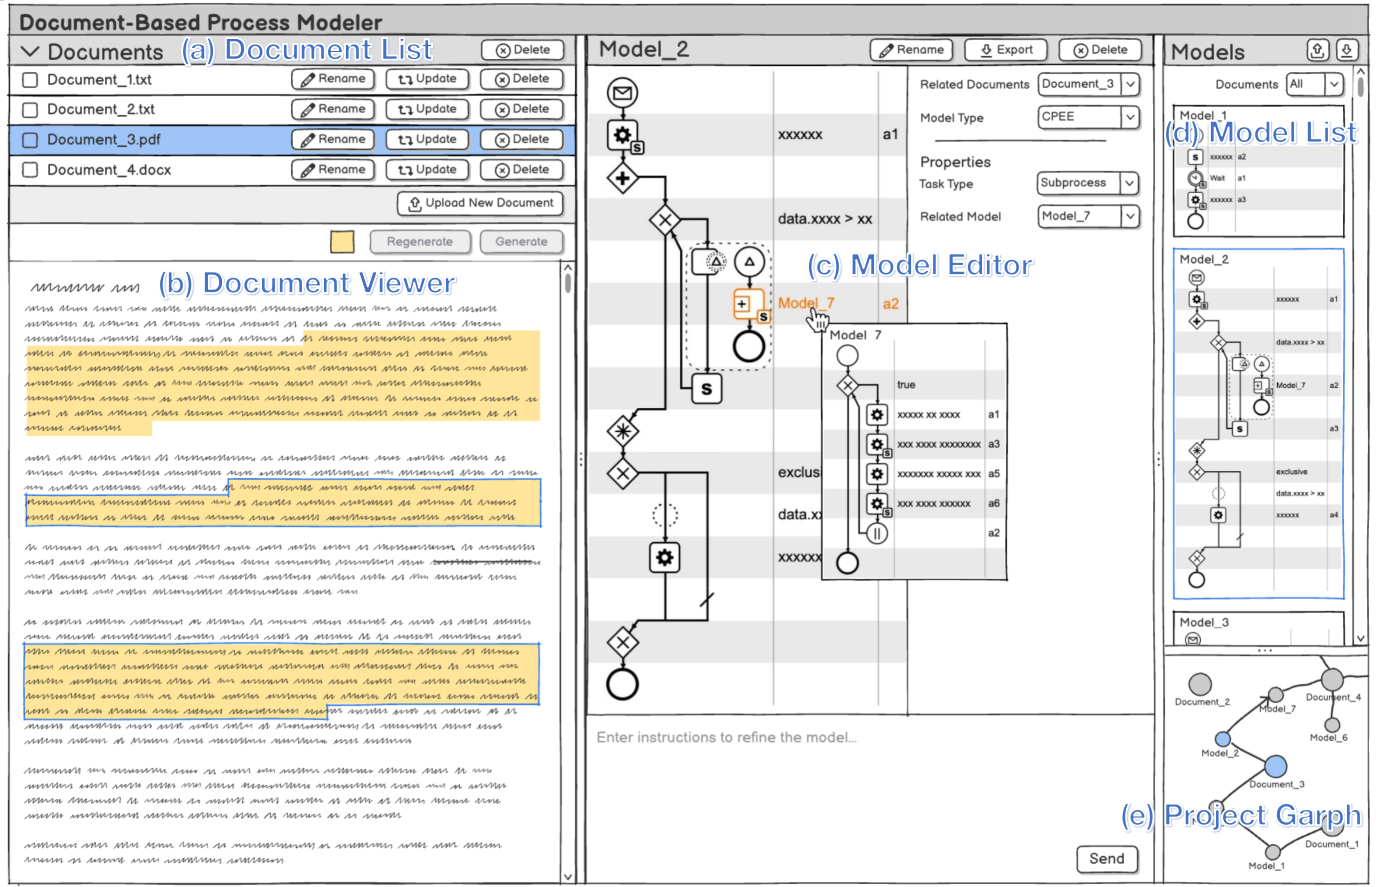
\includegraphics[width=0.9\textwidth]{images/mock-up.png}
    \label{fig:sol_ui}
\end{figure}



\section{System Architecture}

The system architecture is illustrated in Figure~\ref{fig:sol_architecture}. It follows a client–server architecture consisting of a frontend, a backend, and a persistence layer, with integration of an external LLM service. The frontend is implemented as a multi-page application (MPA), consisting of a home page, a workspace page, and a statistics page, where the workspace page represents the core of the system, supporting document handling and process model generation. For LLM-based model generation, the frontend sends requests to the external LLM service directly, and the generated results are returned to the frontend for user review and interaction. After user confirmation, the data is transmitted to the backend for persistence. The frontend communicates with the backend via RESTful APIs, through which the backend manages projects, documents, and models and handles data storage. The persistence layer follows a hybrid approach: the actual content of documents and models is stored in the local file system, while their metadata (e.g., version numbers and names) and application data, such as project information and relationships between process models, are maintained in a database.

\begin{figure}[htb!]
    \centering
    \caption{System architecture} 
    
\includegraphics[width=0.8\textwidth]{images/sol_architecture.png}
    \label{fig:sol_architecture}
\end{figure}
